\documentclass[10pt]{article}
\usepackage[polish]{babel}
\usepackage[utf8]{inputenc}
\usepackage[T1]{fontenc}
\usepackage{amsmath}
\usepackage{amsfonts}
\usepackage{amssymb}
\usepackage[version=4]{mhchem}
\usepackage{stmaryrd}
\usepackage{graphicx}
\usepackage[export]{adjustbox}
\graphicspath{ {./images/} }

\title{GIMNAZJUM }

\author{}
\date{}


\begin{document}
\maketitle
\begin{enumerate}
  \item Znajdź wszystkie pary liczb całkowitych \((x, y)\) spełniające równanie:
\end{enumerate}

\[
x^{4}=y^{4}+1223334444
\]

\begin{enumerate}
  \setcounter{enumi}{1}
  \item Na okręgu o promieniu 1 opisano trójkąt prostokątny \(A B C\) o kącie prostym przy wierzchołku \(C\). Na przeciwprostokątnej \(A B\) tego trójkąta wybrano takie punkty \(D\) i \(E\), że zachodzą równości \(A D=A C\) i \(B E=B C\). Oblicz długość odcinka \(D E\).
  \item Udowodnij, że dla liczb dodatnich \(a\) i \(b\) zachodzą nierówności:
\end{enumerate}

\[
\sqrt{\frac{a^{2}+b^{2}}{2}} \geq \frac{a+b}{2} \geq \sqrt{a b} \geq \frac{2}{\frac{1}{a}+\frac{1}{b}}
\]

\section*{LICEUM}
\begin{enumerate}
  \item W kwadracie \(A B C D\) wybieramy na boku \(B C\) taki punkt \(E\), a na boku \(C D\) taki punkt \(F\), że \(|E F|=|B E|+|F D|\). Udowodnij, że kąt \(E A F\) ma \(45^{\circ}\).\\
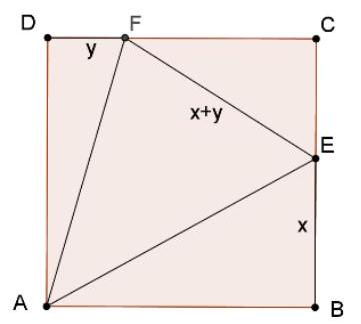
\includegraphics[max width=\textwidth, center]{2024_11_21_76d6cd89e909e377064fg-1}
  \item Pole powierzchni wielościanu opisanego na kuli o promieniu 1 wynosi 12 . Oblicz objętość tego wielościanu.
  \item Liczba rzeczywista \(x\) spełnia równanie \(x^{3}+4 x=8\). Znajdź wartość wyrażenia \(x^{7}+64 x^{2}\).
\end{enumerate}

\end{document}